\documentclass[letterpaper]{article}
\usepackage[submission]{aaai2026}
\usepackage{times}
\usepackage{helvet}
\usepackage{courier}
\renewcommand{\ttdefault}{cmtt}
\usepackage[hyphens]{url}
\usepackage{graphicx}
\urlstyle{rm}
\def\UrlFont{\rm}
\usepackage{natbib}
\usepackage{caption}
\usepackage{amsmath,amssymb,amsthm}
\usepackage{booktabs}
\usepackage{algorithm}
\usepackage{algpseudocode}
\frenchspacing
\setlength{\pdfpagewidth}{8.5in}
\setlength{\pdfpageheight}{11in}
\pdfinfo{
/TemplateVersion (2026.1)
}

\newcommand{\WMC}{\ensuremath{\mathrm{WMC}}}
\newcommand{\tw}{\ensuremath{\mathrm{tw}}}
\newcommand{\R}{\mathbb{R}}
\newcommand{\bC}[1]{\boldsymbol{#1}}
\newif\ifincludesupplement
\includesupplementfalse
\newcommand{\suppref}[1]{\ifincludesupplement Appendix~\csname ref\endcsname{#1}\else technical appendix\fi}
\newtheorem{theorem}{Theorem}
\newtheorem{definition}{Definition}
\newtheorem{proposition}{Proposition}
\newtheorem{example}{Example}

\title{Scaling Ontology-Conditioned Weighted Model Counting with Modular Separators}
\author{
    Anonymous Submission
}
\affiliations{
    Anonymous Institution\\
}
\newcommand{\stitle}[1]{\vspace{1mm}\noindent\textit{#1}}

\begin{document}
\maketitle

\begin{abstract}
Weighted model counting (WMC) turns label-wise predictor scores into a
normalized posterior over assignments that satisfy an ontology, but
monolithic exact inference concentrates its cost in high-width
reconvergent regions. We introduce modular separator WMC, which separates
this cost from the rest of the ontology. Peripheral modules are eliminated
into joint boundary factors, a reduced core is contracted once, and module
marginals are recovered from calibrated boundary posteriors. Exact
separators preserve the monolithic WMC posterior. For wide interfaces,
boundary-conditioned module-WMC queries construct nonnegative
tensor-train (TT) separators that are contracted with the reduced core
without materializing dense tables. This gives a single all-term posterior
layer whose exact and approximate modes share the same separator interface:
exact factors recover monolithic WMC, while TT factors carry
rank-controlled boundary dependence. Experiments on biomedical ontologies
show exact recovery wherever monolithic references are available,
completion of all requested ontology-term marginals on complete
vocabularies, and systematic reduction in recovered-marginal error as
separator rank increases.
\end{abstract}

\section{Introduction}
\label{sec:intro}

Many prediction and reasoning systems assign local scores to Boolean
variables whose joint assignments must satisfy hard symbolic constraints.
This setting includes hierarchical multi-label classification, where labels
follow a taxonomy, and neuro-symbolic models, where neural concept scores
are coupled by a logical theory
\citep{silla2011survey,giunchiglia2020chmcnn,
xu2018semanticloss,ahmed2022spl}. A vector of local scores leaves the
dependence induced by the theory unspecified. Under an independent-product
interpretation, it generally assigns probability mass to invalid
configurations and does not define a normalized distribution over valid
ones.

Existing methods incorporate constraints through ontology-aware
architectures, constraint-based losses, posterior regularization,
constrained decoding, or post-processing
\citep{giunchiglia2020chmcnn,kulmanov2018deepgo,
kulmanov2022deepgozero,ganchev2010posterior,
diligenti2017semantic,xu2018semanticloss,wang2023regularization}.
We study weighted model counting (WMC) as a plug-in hard-constraint
inference layer for fixed predictor scores. Given a Boolean theory and
nonnegative literal weights, WMC sums the weights of its satisfying
assignments \citep{chavira2008wmc}. Interpreting predictor scores as
Bernoulli literal weights and normalizing the count conditions the product
reference distribution on the theory. The resulting posterior has support
only on valid assignments, and every corrected marginal and Boolean query
uses the same normalizer. This probabilistic semantics motivates
our focus on WMC.

Ontology-conditioned prediction is an important large-scale instance.
Protein-function predictors assign scores to Gene Ontology (GO) terms,
whose molecular-function, biological-process, and cellular-component
vocabularies form large directed acyclic graphs
\citep{ashburner2000go,geneontology2023}; anatomy and chemical prediction
use ontologies such as UBERON and ChEBI
\citep{mungall2012uberon,hastings2016chebi}. Figure~\ref{fig:task}(a--b)
illustrates how WMC conditions local protein-function scores on such
ontology relations. These vocabularies combine fixed per-concept scores,
hard semantic constraints, and the scale that stresses exact inference.

\begin{figure}[t]
    \centering
    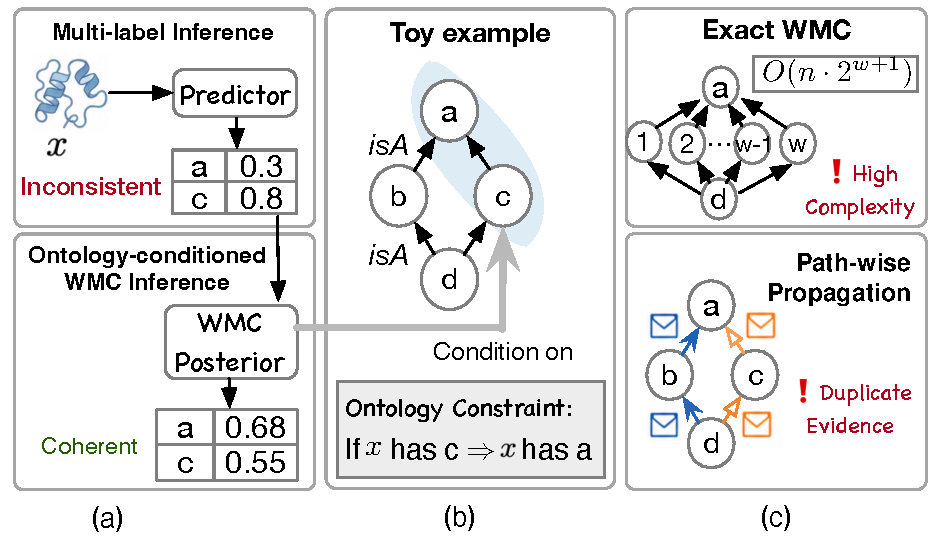
\includegraphics[width=\columnwidth]{intro-aaai.pdf}
    \caption{Ontology-conditioned inference and its bottleneck. (a) WMC restores consistency. (b) Running ontology fragment. (c) Monolithic WMC is width-dependent, while path-wise updates duplicate shared evidence.}
    \label{fig:task}
\end{figure}

\stitle{The Scalability Gap.}
However, implementing this posterior with exact WMC is computationally
difficult. Exact WMC is \#P-hard in general, and practical approaches based
on knowledge compilation or variable elimination can require time and
memory exponential in the structural width of the constraint graph
\citep{bodlaender1993treewidth,darwiche2002kcmap,
darwiche2011sdd,dudek2020addmc,dudek2020dpmc}.
Large ontologies also contain many reconvergent regions, where paths split
through intermediate labels and meet again at shared ancestors. Local or
path-wise propagation provides a cheaper alternative to whole-theory exact
inference, but messages arriving along different paths may depend on shared
evidence. Treating those messages independently can change the posterior
defined by global WMC, as illustrated in Figure~\ref{fig:task}(c). The
scalability challenge is therefore twofold:
avoid monolithic inference over the full ontology, while preserving the
dependencies required by the conditioned-WMC posterior.



\stitle{Our Solution.}
We introduce \emph{modular separator WMC} to address both requirements.
Our key idea is to exploit ontology modularity: eliminate tractable
peripheral modules independently, summarize their joint effects at the
boundary, and restrict the global contraction to a reduced core. Exact
joint separators preserve the global WMC posterior; direct nonnegative TT
separators extend the pipeline to wide boundaries with rank-controlled
approximation. To our knowledge, this is the first framework to scale
ontology-conditioned WMC to complete biomedical ontologies while returning
posterior marginals for every term.
To summarize, the contributions of this paper are:
\begin{itemize}
    \item We introduce modular separator WMC, a boundary-aware framework
    that moves most ontology variables out of the global contraction while
    retaining their joint influence through boundary factors.

    \item We construct wide separators directly from conditioned module-WMC
    queries, separate logical support from a nonnegative TT fit, and inject
    the TT cores into reduced-core inference.

    \item We prove exact recovery for exact separator factors and stability
    of module recovery, validate numerical exactness on full GO cellular
    component and 432 reference subgraphs, and demonstrate all-term
    inference on complete GO, UBERON, and ChEBI vocabularies containing up
    to 205,592 terms.
\end{itemize}


\section{Related Work}
\label{sec:related-work}

\paragraph{Constrained prediction.}
Hierarchical multi-label and neuro-symbolic methods incorporate logical
constraints through structured architectures, constrained losses, posterior
regularization, decoding, or post-processing
\citep{silla2011survey,giunchiglia2020chmcnn,ganchev2010posterior,
diligenti2017semantic,xu2018semanticloss,wang2023regularization,
ahmed2022spl}. We study inference-time probabilistic correction: predictor
scores are fixed, and the objective is to compute marginals under one
normalized distribution over assignments that satisfy the theory.

\paragraph{Weighted and compositional model counting.}
Knowledge compilation and variable elimination support exact WMC, but
their cost can be exponential in structural width
\citep{chavira2008wmc,darwiche2002kcmap,darwiche2011sdd,
dudek2020addmc,dudek2020dpmc,bodlaender1993treewidth}. Compositional WMC
reduces this cost by partitioning a model and communicating through
separators \citep{dal2017partitioned,dal2021compositional}, while ontology
modularity studies logically meaningful decompositions
\citep{cuencagrau2008modular,delvescovo2011atomic}. Our framework
specializes these ideas to predictor-weighted ontology theories through
boundary-aware core selection, recursive contraction, wide joint
separators, and recovery of every ontology-term marginal.

\paragraph{Low-rank separator representations.}
Low-rank tensors support inference in graphical models and
probability-potential operations
\citep{oseledets2011tt,oseledets2010ttcross,
novikov2014mrf,wrigley2017tensorbp,ducamp2020lowrank}. We construct
nonnegative TT separators directly from boundary-conditioned module-WMC
queries, project logical support separately, and retain the TT
representation during reduced-core inference.


\section{Preliminaries}
\label{sec:preliminaries}

\paragraph{Problem Setup.}
We fix an input \(x\) and suppress it in the notation. Let
\(Y=\{1,\ldots,m\}\) index the ontology terms. For each ontology term
\(i\in Y\), the Boolean variable \(y_i\in\{0,1\}\) indicates whether
term \(i\) is assigned to \(x\). A trained predictor provides a score
\(p_i\in(0,1)\); endpoint scores are clipped before inference so that all
literal weights remain positive. We use \(p_i\) as the weight of \(y_i=1\)
and \(1-p_i\) as the weight of \(y_i=0\). For a complete assignment
\(y=(y_1,\ldots,y_m)\), the resulting product weight is
\[
q_p(y)
=
\prod_{i=1}^m p_i^{y_i}(1-p_i)^{1-y_i}.
\]
We interpret the label-wise scores as Bernoulli parameters and use
\(q_p\) as a product reference distribution. This modeling choice defines
the joint distribution conditioned by WMC. The guarantees below concern
conditioning of \(q_p\) on the ontology; calibration to the data
distribution is evaluated empirically.

The ontology restricts which complete assignments are valid. We write
these constraints as a Boolean formula \(T\) over the variables
\(\{y_i:i\in Y\}\). For an \texttt{is-a} edge from child \(c\) to
parent \(\pi\), \(T\) contains the implication
\[
y_c \Rightarrow y_\pi .
\]
Additional grounded Horn clauses can be added to \(T\) when present in
the ontology. The factorization results below apply to any finite Boolean
factor graph satisfying the stated partition condition. The empirical
ontology experiments in this paper use binary child-to-parent
implications derived from \texttt{is-a} edges. A complete assignment
\(y\) is valid when it satisfies \(T\), written \(y\models T\).

\paragraph{Weighted model counting.}
Weighted model counting sums the weights of complete Boolean assignments
that satisfy a Boolean formula \citep{chavira2008wmc}. In this paper,
the formula is \(T\), and the assignment weight is \(q_p(y)\). The
normalizing constant is
\[
Z_T(p)
=
\mathrm{WMC}(T,p)
=
\sum_{y\models T} q_p(y).
\]
Conditioning on the ontology gives
\[
p_T(y)
=
\frac{\mathbf{1}[y\models T]\,q_p(y)}
     {Z_T(p)},
\]
where \(\mathbf{1}[\cdot]\) is the indicator function. The target
marginal for ontology term \(i\) is
\[
\mu_i
=
p_T(y_i=1)
=
\frac{\mathrm{WMC}(T\wedge y_i,p)}
     {\mathrm{WMC}(T,p)}.
\]
These marginals are the reference quantities throughout the paper.

\paragraph{Constraint graphs and treewidth.}
The constraint graph \(G_T\) has one node for each Boolean variable. Two
variables are adjacent in \(G_T\) when they occur together in a clause
of \(T\). Exact variable elimination and junction tree inference process
groups of variables jointly. For binary variables, their cost is
exponential in the induced width of the chosen elimination order
\citep{pearl1988probabilistic,bodlaender1993treewidth}. Let
\(\widehat w(G)\) denote the min-fill induced width used in our
implementation; it is a heuristic upper bound on
\(\operatorname{tw}(G)\). For \(S\subseteq Y\), we write
\(\widehat w(S)=\widehat w(G_T[S])\). This width dependence is the
structural bottleneck for exact WMC on large ontologies.

\paragraph{Core variables, modules, and boundaries.}
Given a constraint graph \(G_T=(Y,E_T)\), our method will select a subset
of variables \(C\subseteq Y\). We call \(C\) the core. The variables in
\(C\) remain after the module variables are eliminated. Once \(C\) is fixed,
the modules are defined as the connected components of the graph obtained
by removing \(C\):
\[
M_1,\ldots,M_s
=
\operatorname{ConnComp}(G_T\setminus C).
\]
Thus modules are not independent input objects. They are determined by
the selected core.

For each module \(M_j\), we define its boundary as the set of adjacent
core variables,
\[
B_j
=
\{c\in C : (c,m)\in E_T \text{ for some } m\in M_j\}.
\]
The boundary variables remain in the core, but they are included when the
module is eliminated. The augmented module is
\[
A_j = M_j\cup B_j .
\]
Thus \(B_j\) contains core variables adjacent to \(M_j\), not variables
eliminated inside \(M_j\). It is the interface through which the module
affects the computation over \(C\). We use \(\widehat w(A_j)\) as an
unrestricted structural diagnostic. It is not, by itself, the width of
forming a separator factor because an unrestricted order may eliminate
boundary variables.

For separator construction, let \(\Pi(M_j)\) be the elimination orders
that eliminate only \(M_j\), leaving every variable in \(B_j\)
uneliminated. The boundary-constrained width is
\[
w_j^\partial
=
\min_{\pi\in\Pi(M_j)}
\max_{v\in M_j}
\left(
\left|\operatorname{scope}(f_v^\pi)\right|-1
\right),
\]
where \(f_v^\pi\) is the intermediate factor produced when eliminating
\(v\) under order \(\pi\). We write \(\widehat w_j^\partial\) for the
corresponding boundary-last min-fill upper bound used operationally.

\section{Motivation: Reconvergent Dependence}
\label{sec:local-reconvergence}

The WMC target is defined by a global sum over valid complete assignments.
A directed path-wise update agrees with this target on non-reconvergent
tree fragments, but reconvergent paths can carry evidence from a shared
source and change the resulting posterior.
Consider the diamond fragment
\[
T_{\diamond}
=
(y_d \Rightarrow y_b)
\wedge
(y_d \Rightarrow y_c)
\wedge
(y_b \Rightarrow y_a)
\wedge
(y_c \Rightarrow y_a),
\]
with
\[
p_a=p_b=p_c=p_d=\frac{1}{2}.
\]
Exact WMC counts valid complete assignments once and gives
\[
p_{T_{\diamond}}(y_a=1)=\frac{5}{6}.
\]
A path-wise calculation propagates the evidence from \(d\) through
\(b\) and \(c\) independently and gives
\[
\widehat{\mu}_a
=
\frac{9}{10}.
\]
The two values differ because the paths \(d\to b\to a\) and
\(d\to c\to a\) share \(d\), while the final update treats their messages
as independent. The arithmetic is given in \suppref{app:diamond-calculation}. An
eliminated region that touches several retained variables must therefore
be summarized by a joint boundary factor.

\section{Modular Separator WMC}
\label{sec:method}

\paragraph{Overview.}
Given the core, modules, and boundaries defined above, the method
eliminates each module while retaining its boundary, producing one joint
separator factor. These factors are contracted with the core, and saved
module calibrations recover all eliminated marginals in reverse order.
Exact separators preserve the WMC target; wide separators are retained in
factorized TT form. Figure~\ref{fig:method} summarizes the computation.

\begin{figure*}[t]
\centering
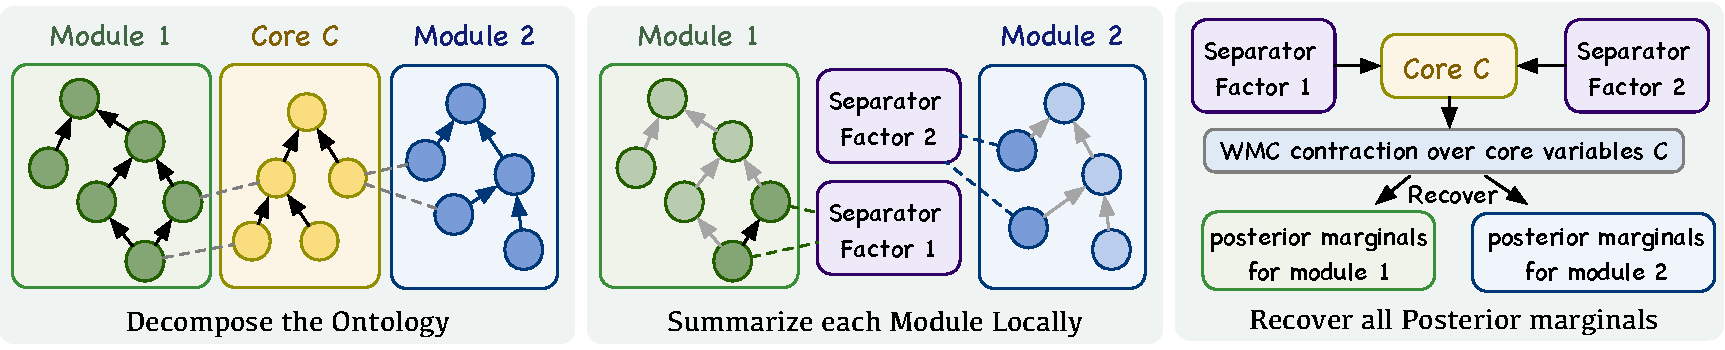
\includegraphics[width=\textwidth]{method.pdf}
\caption{Modular separator WMC. Modules are eliminated into separator factors \(F_j(y_{B_j})\); WMC over the core variables \(C\) then supports posterior recovery inside each module.}
\label{fig:method}
\end{figure*}

\paragraph{Choosing the core.}
The exact construction below applies to any fixed core \(C\). In our
selector, variables receive the static lexicographic score
\[
s(v)=\bigl(\deg_{G_T}(v),\,d_{\mathrm{mp}}(v),\,\operatorname{id}(v)\bigr),
\]
where \(d_{\mathrm{mp}}(v)\) is the number of \texttt{is-a} parents of
\(v\), and the identifier breaks ties deterministically.
Algorithm~\ref{alg:core-selection} adds variables in batches of
\(k=\max(1,\lceil\beta|Y|\rceil)\), recomputes modules and boundary-last
width estimates, and returns after all modules satisfy the cap or the core
budget is exhausted. The selector affects computational cost; the exactness
results apply to any decomposition satisfying the factor partition.

\begin{algorithm}[t]
\caption{Boundary-aware core selection}
\label{alg:core-selection}
\small
\begin{algorithmic}[1]
\Require \(G_T\), width cap \(w_{\max}\), batch fraction \(\beta\), core budget \(\rho\)
\State \(C\gets\varnothing\); rank \(Y\) once by decreasing \(s(v)\)
\Loop
  \State \(M_1,\ldots,M_s\gets\operatorname{ConnComp}(G_T\setminus C)\)
  \State form \(B_j\) and estimate \(\widehat w_j^\partial\) for every \(M_j\)
  \If{\(\max_j\widehat w_j^\partial\leq w_{\max}\)}
    \State \Return \(C\)
  \EndIf
  \If{\(|C|+k>\rho|Y|\)}
    \State \Return \textsc{budget-exhausted}
  \EndIf
  \State add the next \(k\) ranked variables to \(C\)
\EndLoop
\end{algorithmic}
\end{algorithm}

\paragraph{Factor partition.}
Let the weighted Boolean theory be written as a product of literal-weight
factors and Boolean constraint factors. After \(C\) is fixed, we partition
these factors into a core part and module parts. Let
\(\Phi_C(y_C)\) contain the literal weights of core variables and all
constraint factors whose variables lie entirely in \(C\). For module
\(M_j\), let \(\Phi_j(y_{M_j},y_{B_j})\) contain the literal weights of
variables in \(M_j\) and all constraint factors assigned to that module.

A constraint factor with at least one variable in \(M_j\) and no
non-core variable outside \(M_j\) is assigned to module \(j\). Because the
\(M_j\) are connected components of \(G_T\setminus C\), no constraint
factor contains non-core variables from two different modules. Hence the
full weighted theory factorizes as
\[
\Phi(y)
=
\Phi_C(y_C)
\prod_{j=1}^{s}
\Phi_j(y_{M_j},y_{B_j}).
\]

\paragraph{Exact separator elimination.}
For each module, we eliminate the module variables while leaving the
boundary variables uneliminated:
\[
F_j(y_{B_j})
=
\sum_{y_{M_j}}
\Phi_j(y_{M_j},y_{B_j}).
\]
We call \(F_j\) the separator factor of module \(j\). It is a function of
the full boundary assignment \(y_{B_j}\). When \(|B_j|>1\), \(F_j\) is
joint over all variables in \(B_j\) and retains the dependence induced by
the eliminated module.

For small \(B_j\), \(F_j\) is stored as a dense table. For large
boundaries, this table has \(2^{|B_j|}\) entries. The mathematical object
remains \(F_j\); compact representations approximate its dense table.

\paragraph{Solving over the core variables.}
After eliminating all module variables, the original normalizer can be
evaluated by a WMC contraction over the core variables:
\[
Z_T(p)
=
\sum_{y_C}
\Phi_C(y_C)
\prod_{j=1}^{s}
F_j(y_{B_j}).
\]
The remaining variables are \(C\), and the remaining factors are
\(\Phi_C\) and one \(F_j\) for each eliminated module. When every
separator factor is exact, this contraction has the same normalizer as
monolithic WMC. Solving it gives posterior marginals
\(p_T(y_c=1)\) for \(c\in C\) and, for each module, the joint posterior
distribution \(p_T(y_{B_j})\). When \(B_j\) contains multiple variables,
this is a distribution over the full boundary assignment, not separate
one-variable marginals.

\paragraph{Recursive contraction.}
If the reduced core exceeds the width cap, the same construction is
applied recursively to its factor graph. Existing factors that span
several candidate modules force those modules to be merged, preserving the
factor partition. Calibrations are stored at each level; after solving the
terminal core, boundary posteriors are propagated backward to recover all
singleton marginals. Recursive inference is exact when every separator is
exact and approximate otherwise.

\paragraph{Recovering posterior marginals inside modules.}
For boundary assignments with \(F_j(y_{B_j})>0\), define the exact module
conditional
\[
K_j(y_{M_j}\mid y_{B_j})
=
\frac{\Phi_j(y_{M_j},y_{B_j})}{F_j(y_{B_j})}.
\]
Boundary assignments with \(F_j(y_{B_j})=0\) have zero module mass and do
not contribute to the exact posterior. For each \(i\in M_j\), define the
conditional single-variable marginal
\[
h_{j,i}(b)
=
\frac{
\sum_{y_{M_j}:y_i=1}
\Phi_j(y_{M_j},b)
}{
F_j(b)
}.
\]
The required posterior marginal is
\[
\mu_i
=
\sum_b h_{j,i}(b)\,p_T(y_{B_j}=b).
\]
Thus the algorithm need not materialize the full joint distribution over
\(M_j\). A calibrated module junction tree reuses its messages to extract
the required conditional singleton marginals for all \(i\in M_j\).

\paragraph{Direct tensor-train separators.}
When \(B_j=(b_1,\ldots,b_k)\) is large, the dense table for \(F_j\) has
\(2^k\) entries. We query its entries without constructing that table:
\[
\mathcal O_j(b)
=
\sum_{y_{M_j}}\Phi_j(y_{M_j},b)
=F_j(b),
\]
where each oracle call clamps \(B_j=b\) and performs exact WMC inside the
module. Let \(\mathcal Q_j\) be a set of sampled boundary assignments and
\(N_j=|\mathcal Q_j|\). We evaluate the oracle on \(\mathcal Q_j\) and
fit the supported positive entries with the nonnegative rank-\(r\)
tensor train
\[
\widehat V_{j,r}(b)
=
G_1[b_1]G_2[b_2]\cdots G_k[b_k],
\qquad G_\ell[b_\ell]\geq 0,
\]
using alternating least squares with nonnegative least-squares core
updates. Optimization hyperparameters and validation protocols are reported
with the experimental setup; the full optimization protocol is given in
\suppref{app:direct-tt-optimization}.

Logical support is kept separate from the fitted positive values. Let
\(T_j\) contain the Boolean constraints assigned to module \(j\). Define
\begin{align*}
S_j(b)
&=\mathbf{1}\!\left[
\exists y_{M_j}:T_j(y_{M_j},b)
\right],\\
\widehat F_{j,r}(b)
&=S_j(b)\widehat V_{j,r}(b).
\end{align*}
For the implication theories used here, reachability within \(M_j\cup B_j\)
yields the implied boundary-to-boundary constraints, which are injected as
Boolean factors into the reduced graph.

The TT remains factorized during reduced-core inference. Introducing bond
indices \(\alpha_1,\ldots,\alpha_{k-1}\) turns each TT core into a local
factor
\[
g_\ell(\alpha_{\ell-1},b_\ell,\alpha_\ell)
=G_\ell[b_\ell]_{\alpha_{\ell-1},\alpha_\ell},
\]
with \(\alpha_0=\alpha_k=1\). We inject these factors and \(S_j\) into the
reduced factor graph and eliminate Boolean and bond variables jointly.
This TT-native contraction avoids materializing \(\widehat F_{j,r}\);
rank controls both its representational capacity and the bond-state cost.

If approximate separator factors are supplied, the corresponding
reduced-core contraction is
\[
\widehat{Z}_T(p)
=
\sum_{y_C}
\Phi_C(y_C)
\prod_{j=1}^{s}
\widehat{F}_{j,r}(y_{B_j}).
\]
The exact \(F_j\) remain the reference target; any
\(\widehat F_{j,r}\ne F_j\) makes the resulting posterior approximate.

\paragraph{Exactness and recovery stability.}
The first result states that exact separator factors preserve monolithic
WMC.

\begin{proposition}[Exact modular contraction]
\label{prop:exact-modular}
Under the factor partition above,
\[
Z_T(p)
=
\sum_{y_C}
\Phi_C(y_C)
\prod_{j=1}^{s}
F_j(y_{B_j}).
\]
If every separator factor \(F_j\) is exact, then the posterior marginals
of variables in \(C\) and those recovered for variables in \(M_j\)
through \(K_j\) equal the corresponding monolithic WMC marginals.
\end{proposition}

The proof is a reordering of the sum-product computation. The module
interiors are disjoint, every original factor appears exactly once, and
summing out module variables before summing over \(C\) gives the same
result as summing over all variables together.

The second guarantee bounds recovery error by boundary-posterior error;
\(\mathrm{TV}\) denotes total-variation distance.

\begin{proposition}[Stability of module recovery]
\label{prop:boundary-error}
Assume that \(B_j\) separates \(M_j\) from the remaining variables in the
factor graph. Let \(\widehat{p}(y_{B_j})\) approximate the joint posterior
distribution over \(B_j\), with
\[
\operatorname{supp}\widehat p(y_{B_j})
\subseteq
\{b:F_j(b)>0\}.
\]
Define
\[
\widehat{p}(y_{M_j})
=
\sum_{y_{B_j}}
K_j(y_{M_j}\mid y_{B_j})\,\widehat{p}(y_{B_j}).
\]
Then
\[
\mathrm{TV}\!\left(
\widehat{p}(y_{M_j}),p_T(y_{M_j})
\right)
\le
\mathrm{TV}\!\left(
\widehat{p}(y_{B_j}),p_T(y_{B_j})
\right).
\]
Consequently, the absolute error of any single-label marginal in \(M_j\)
is bounded by the total variation error in the joint posterior
distribution over \(B_j\).
\end{proposition}

The proposition assumes a boundary posterior as input to module
recovery; it is independent of how that boundary posterior is computed.
The proof is given in \suppref{app:boundary-error-proof}.

\paragraph{Computational scope.}
Let \(n_j=|M_j|\), let \(\widehat w_j^\partial\) be the boundary-last
module width, and let \(\widehat w_C\) be the induced width of the
reduced core. Exact dense-mode cost is exponential in these widths and
requires \(2^{|B_j|}\) storage for each dense separator. For a direct TT
separator, let \(\mathcal C_j^\partial\) be the
cost of one boundary-clamped module-WMC query, and let
\(\operatorname{Fit}_j\) denote fitting cost. Construction uses
\[
O\!\left(
\sum_j\!\left[N_j\mathcal C_j^\partial+
\operatorname{Fit}_j(N_j,|B_j|,r)\right]
\right)
\]
time and stores \(O(\sum_j[|B_j|r^2+|R_j|])\) TT parameters and projected
support factors, where \(R_j\) is the set of boundary implications.
Reduced-core cost depends on the joint elimination order over Boolean and
rank-\(r\) bond variables and is evaluated end to end. The dense-mode
expression is given in \suppref{app:dense-cost}.

\section{Experiments}
\label{sec:experiments}

We evaluate target preservation (\textbf{RQ1}), complete-ontology
scalability (\textbf{RQ2}), and fixed-score protein-function prediction
(\textbf{RQ3}).

\subsection{Exp 1: WMC Inference on Ontology Benchmarks}

\paragraph{Datasets.}
We use complete ontology graphs from the three Gene Ontology namespaces:
cellular component (GO cc), molecular function (GO mf), and biological
process (GO bp) \citep{ashburner2000go,geneontology2023}, together with
complete UBERON and ChEBI vocabularies
\citep{mungall2012uberon,hastings2016chebi}. Each ontology term is
one Boolean variable and each child-parent relation is the implication
\(y_c \Rightarrow y_p\). We instantiate score vectors from
uniform, Beta\((2,2)\), Beta\((0.5,0.5)\), and extreme-prior families.

\paragraph{Baselines.}
All methods share the Boolean theory, literal weights, and marginal
queries. Small-instance references use brute force and monolithic
junction-tree (JT) inference. The scale comparison uses the same JT
backend monolithically and inside modules, isolating the effect of
decomposition. Modular WMC uses exact \(F_j\) when enumerable and
rank-controlled TT factors otherwise.

\paragraph{Evaluation metrics.}
Exact-reference metrics are mean absolute error (MAE), maximum
absolute error, and completion. Scale metrics are coverage,
boundary-last width, recursion depth, boundary size, end-to-end
time, and peak memory. TT validation reports separator
total-variation distance (TV), held-out normalized MAE (NMAE),
and recovered-marginal MAE.

\paragraph{Implementation details.}
The operational selector uses Algorithm~\ref{alg:core-selection} with
\(w_{\max}=14\), \(\beta=0.01\), and \(\rho=0.30\); reported widths are
min-fill upper bounds. All rows share the same theory, weights, queries,
and backends. Optimizer settings, BP damping, score clipping,
retained-reference seeds, and hardware allocations are reported in
\suppref{app:reproducibility}.

\paragraph{RQ1: Does modular contraction preserve the WMC target?}
Table~\ref{tab:exactness} compares exact-factor modular WMC with
exact references on full GO cc and 432 retained subgraphs. Numerical
agreement confirms that factor partition, separator elimination, and
module recovery preserve the WMC target.

\begin{table}[t]
\centering
\scriptsize
\setlength{\tabcolsep}{3pt}
\begin{tabular}{lrrr}
\toprule
Benchmark & MAE & Max error & Completed \\
\midrule
Full GO cc & \(1.95{\times}10^{-17}\) & \(3.33{\times}10^{-16}\) & 4,041/4,041 \\
Reference subgraphs & \(2.94{\times}10^{-16}\) & \(1.02{\times}10^{-14}\) & 432/432 \\
\bottomrule
\end{tabular}
\caption{
Exact-factor modular WMC against exact references on full GO cc and
retained subgraphs.
}
\label{tab:exactness}
\end{table}

\paragraph{RQ2: Does decomposition enable ontology-scale inference?}
This experiment tests whether decomposition turns complete-ontology WMC
into all-term posterior recovery at biomedical scale. Each row uses one
complete ontology, one Boolean theory, one score vector, one marginal-query
set, and one resource protocol. Figure~\ref{fig:width-rank}(a) measures the
structural effect of selecting a core before inference, and
Table~\ref{tab:operational-scale} compares monolithic JT with modular WMC
on recovered marginals, wall time, and peak memory.

\begin{table*}[t]
\centering
\scriptsize
\setlength{\tabcolsep}{1.6pt}
\begin{tabular}{lrrrrr|rrr|rrr}
\toprule
\multicolumn{6}{c|}{Structure}
&
\multicolumn{3}{c|}{Monolithic JT}
&
\multicolumn{3}{c}{Modular WMC} \\
\cmidrule(lr){1-6}
\cmidrule(lr){7-9}
\cmidrule(lr){10-12}
Ontology
& Cov.
& \(\max_j \widehat w_j^\partial\)
& Modules
& Max depth
& Max \( |B_j| \)
& Output
& Time
& RSS
& Output
& Time
& RSS \\
\midrule
GO cc
& 100.0\%
& 12
& 1
& 0
& 0
& 4,041/4,041
& 2.4\,s
& 1.1
& 4,041/4,041
& 14.8\,s
& 1.6 \\

GO mf
& 95.0\%
& 5
& 6,519
& 4
& 176
& OOM
& 18.6\,min
& 300
& 10,131/10,131
& 3.2\,min
& 8.7 \\

GO bp
& 91.0\%
& 12
& 7,249
& 8
& 624
& OOM
& 7.3\,min
& 300
& 25,950/25,950
& 28.4\,min
& 31.4 \\

UBERON
& 95.0\%
& 11
& 8,427
& 6
& 391
& OOM
& 11.1\,min
& 300
& 14,977/14,977
& 8.6\,min
& 16.2 \\

ChEBI
& 98.0\%
& 12
& 181,679
& 12
& 1,082
& OOM
& 2.8\,min
& 300
& 205,592/205,592
& 9.7\,h
& 126 \\
\bottomrule
\end{tabular}

\caption{
Whole-ontology structure and matched all-term inference.
Cov.\ is \(\sum_j |M_j|/|Y|\), and the reported width is the
top-level maximum boundary-last width. Output is either the number
of recovered marginals or OOM at the 300\,GB limit. Time includes
preprocessing, inference, and posterior recovery; RSS is peak resident set
size in GB.
}
\label{tab:operational-scale}
\end{table*}

The result separates the structural and inferential effects of
decomposition. Core selection turns the complete ontologies into tractable
module eliminations, and the modular contraction returns all requested
posterior marginals across the benchmark suite. Monolithic JT serves as the
same-semantics reference where structural width is small and as the
resource-limited comparison where width is concentrated. The large
recursive boundaries in the modular runs are the target of the wide
separator validation in Table~\ref{tab:direct-tt}.

\paragraph{Mechanism: Direct TT separator validation.}
Figure~\ref{fig:width-rank}(b) isolates representational capacity using
the exact joint. Table~\ref{tab:direct-tt} evaluates the query-fitted
construction used by the pipeline in two regimes: enumerable reference
modules and production wide separators. On enumerable reference modules,
exact dense separators provide ground-truth separator and
recovered-marginal errors. On production wide separators, whose dense
tables are infeasible, we report error on independent
boundary-conditioned module-WMC queries. All fitted methods use the same
training queries at a given validation instance.

\begin{figure}[t]
\centering
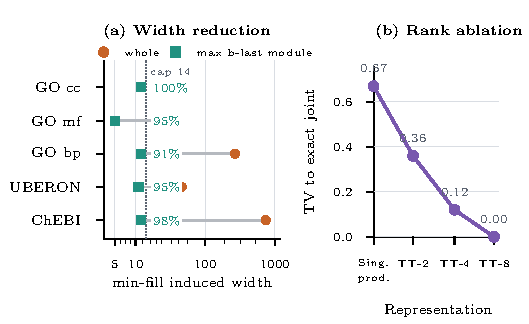
\includegraphics[width=\columnwidth]{fig_width_rank.pdf}
\caption{Structural and separator diagnostics. (a) Whole-theory min-fill
width versus the top-level maximum boundary-last module width. (b)
Exact-joint representation error on one enumerated 10-variable GO cc
separator; singleton product is formed from exact singleton marginals,
while TT-\(r\) denotes the rank-\(r\) tensor-train SVD approximation.}
\label{fig:width-rank}
\end{figure}

\begin{table*}[t]
\centering
\scriptsize
\setlength{\tabcolsep}{2.6pt}
\resizebox{\textwidth}{!}{%
\begin{tabular}{lrrlrrrrr}
\toprule
Validation set
& $n$
& $|B|$
& Metric
& Direct product
& TT-2
& TT-4
& TT-8
& Exact \\
\midrule

\multicolumn{9}{l}{\textit{Exact-reference modules}} \\

GO cc modules
& 24
& 3--9
& Marg.\ MAE
& \(4.11{\times}10^{-2}/8.55{\times}10^{-2}\)
& \(8.42{\times}10^{-3}/2.31{\times}10^{-2}\)
& \(1.37{\times}10^{-3}/4.82{\times}10^{-3}\)
& \(2.84{\times}10^{-4}/9.31{\times}10^{-4}\)
& \(5.00{\times}10^{-16}/9.99{\times}10^{-16}\) \\

GO bp modules
& 24
& 5--12
& Marg.\ MAE
& \(4.79{\times}10^{-2}/3.61{\times}10^{-1}\)
& \(1.12{\times}10^{-2}/5.84{\times}10^{-2}\)
& \(2.46{\times}10^{-3}/1.19{\times}10^{-2}\)
& \(4.73{\times}10^{-4}/2.08{\times}10^{-3}\)
& \(6.66{\times}10^{-16}/2.00{\times}10^{-15}\) \\

$|B|=10$ separator
& 1
& 10
& Sep.\ TV
& 0.241
& 0.108
& 0.028
& 0.006
& 0 \\

$|B|=10$ separator
& 1
& 10
& Marg.\ MAE
& \(1.83{\times}10^{-2}\)
& \(7.36{\times}10^{-3}\)
& \(1.92{\times}10^{-3}\)
& \(6.81{\times}10^{-4}\)
& \(2.07{\times}10^{-15}\) \\

\midrule
\multicolumn{9}{l}{\textit{Production wide separators}} \\

GO mf
& 32
& 24--176
& Val.\ NMAE
& \(1.26{\times}10^{-1}/3.18{\times}10^{-1}\)
& \(3.84{\times}10^{-2}/1.07{\times}10^{-1}\)
& \(1.21{\times}10^{-2}/3.42{\times}10^{-2}\)
& \(3.40{\times}10^{-3}/9.80{\times}10^{-3}\)
& -- \\

GO bp
& 41
& 31--624
& Val.\ NMAE
& \(1.78{\times}10^{-1}/4.26{\times}10^{-1}\)
& \(5.73{\times}10^{-2}/1.54{\times}10^{-1}\)
& \(2.07{\times}10^{-2}/5.91{\times}10^{-2}\)
& \(6.80{\times}10^{-3}/1.87{\times}10^{-2}\)
& -- \\

UBERON
& 35
& 27--391
& Val.\ NMAE
& \(1.51{\times}10^{-1}/3.72{\times}10^{-1}\)
& \(4.61{\times}10^{-2}/1.29{\times}10^{-1}\)
& \(1.63{\times}10^{-2}/4.70{\times}10^{-2}\)
& \(5.10{\times}10^{-3}/1.43{\times}10^{-2}\)
& -- \\

ChEBI
& 58
& 46--1,082
& Val.\ NMAE
& \(2.03{\times}10^{-1}/4.91{\times}10^{-1}\)
& \(7.42{\times}10^{-2}/1.88{\times}10^{-1}\)
& \(2.91{\times}10^{-2}/7.34{\times}10^{-2}\)
& \(9.70{\times}10^{-3}/2.46{\times}10^{-2}\)
& -- \\

\bottomrule
\end{tabular}
}
\caption{
Direct TT separator validation. \(n\) counts evaluated separator--score
instances and \(|B|\) gives the boundary-size range. Exact-reference rows
report median/maximum recovered-marginal MAE; the enumerated separator
additionally reports TV to the normalized exact joint. Production rows
report median/maximum held-out NMAE. Direct product and TT-\(r\) use
matched queries; Exact is unavailable without dense enumeration.
}
\label{tab:direct-tt}
\end{table*}

The exact-reference results show that increasing direct-TT rank
reduces both separator error and the error propagated to recovered
marginals. The production results establish that the same trend
persists on the wide interfaces encountered by complete-ontology
inference, where exact dense validation is unavailable. Direct-product
factors remain inaccurate despite preserving logical support,
indicating that completion in Table~\ref{tab:operational-scale}
depends on retaining joint boundary dependence rather than only
decomposing the theory.

\subsection{Exp 2: Downstream: Protein-Function Prediction}

\paragraph{Datasets.}
We use the Critical Assessment of Function Annotation (CAFA)
protein-function benchmark
\citep{radivojac2013cafa,zhou2019cafa3}.
Protein annotations are mapped to the GO snapshot used by the
inference experiments, yielding 5,969 proteins evaluated on the
complete 4,041-term GO cc namespace.

\paragraph{Implementation details.}
A fixed DeepGO-style multilayer perceptron (MLP) and
DeepGOPlus-style convolutional neural network (CNN)
\citep{kulmanov2018deepgo,kulmanov2020deepgoplus}
produce one score for every protein--term pair. Predictor parameters
and raw scores are held fixed across all post-processing methods.
Table~\ref{tab:downstream} denotes the two score sources as MLP and
DeepGOCNN.

\paragraph{Baselines.}
We compare the raw predictor scores with upward max closure
\citep{obozinski2008consistent,giunchiglia2020chmcnn}
and synchronous loopy sum-product belief propagation (BP)
\citep{pearl1988probabilistic}. The exact-WMC row uses junction-tree
(JT) calibration on the complete GO cc constraint graph, matching the
namespace for which monolithic exact inference is available.

\paragraph{Evaluation metrics.}
Following the CAFA evaluation protocol, we report the maximum
protein-centric F-score over thresholds (F$_{\max}$), mean area under
the precision--recall curve (mAUPR), minimum semantic distance over
thresholds (S-min), Brier score, expected calibration error (ECE),
and true-path violation rate (Viol.).

\paragraph{RQ3: Does ontology-conditioned WMC provide
fixed-score posterior correction?}
Table~\ref{tab:downstream} holds the predictors and evaluation set
fixed, changing only ontology-conditioned inference. Across both
score sources, exact WMC yields zero true-path violations and the lowest
Brier and ECE among constraint-enforcing methods, while remaining
comparable to loopy BP on ranking metrics. This isolates the effect of
posterior correction from retraining or model selection.

\begin{table}[t]
\centering
\scriptsize
\setlength{\tabcolsep}{1.2pt}
\begin{tabular}{lrrrrrr}
\toprule
Method
& F$_{\max}$
& mAUPR
& S-min
& Brier
& ECE
& Viol. \\
\midrule

\multicolumn{7}{l}{\textit{DeepGOCNN}} \\

Raw
& 0.55396
& 0.03925
& 16.298
& 0.002338
& 0.000938
& 0.03974 \\

Max closure
& 0.62239
& 0.03809
& 16.948
& 0.002690
& 0.001758
& 0 \\

Loopy BP
& 0.65439
& 0.04079
& 15.131
& 0.002020
& 0.001247
& 0 \\

Exact WMC (JT)
& 0.65495
& 0.04075
& 15.133
& 0.002016
& 0.001234
& 0 \\

\addlinespace

\multicolumn{7}{l}{\textit{MLP}} \\

Raw
& 0.58606
& 0.17905
& 14.219
& 0.002159
& 0.001048
& 0.06813 \\

Max closure
& 0.65461
& 0.17841
& 15.658
& 0.002364
& 0.001614
& 0 \\

Loopy BP
& 0.67037
& 0.16367
& 14.015
& 0.001952
& 0.001337
& \(1.45{\times}10^{-7}\) \\

Exact WMC (JT)
& 0.67079
& 0.16326
& 14.014
& 0.001947
& 0.001324
& 0 \\

\bottomrule
\end{tabular}
\caption{
Post-processing fixed DeepGOCNN and MLP scores on complete GO cc.
Higher is better for F$_{\max}$ and mAUPR; lower is better for all
other metrics.
}
\label{tab:downstream}
\end{table}



\section{Conclusion and Limitations}\label{sec:conclusion}
% Modular separator WMC turns ontology-conditioned WMC into a scalable
% all-term posterior inference operator. The method eliminates peripheral
% modules into joint separator factors, contracts a reduced core, and
% recovers every module marginal from calibrated boundary posteriors. Exact
% separators recover monolithic WMC, and nonnegative TT separators carry wide
% interfaces through the same reduced-core inference pipeline. Across five
% complete biomedical ontologies, the method returns all-term marginal output
% up to 205,592 terms, and the GO cc application shows normalized,
% constraint-satisfying posterior scores for fixed protein-function
% predictors.

We introduced a modular-separator framework for scaling weighted
model counting in large constrained probabilistic models. The method
uses exact module elimination and joint separator factors to reduce
global contraction while retaining posterior recovery for all
variables. Exact separators preserve the monolithic WMC target, while
factorized tensor-train separators extend the framework to boundaries
for which dense representation is infeasible. Experiments on complete
biomedical ontologies show that modular decomposition enables
all-term inference beyond monolithic contraction, and the separator
studies confirm the importance of preserving joint boundary
dependence. 

However, the method relies on theories admitting useful modular
decompositions and separators compressible at moderate TT rank.
Approximate separators also lack an a posterior certificate for
marginal error. Future work will address these limitations through
adaptive decomposition, automatic rank selection, and certified
posterior-error bounds.
% However, the method relies on theories that admit useful modular
% decompositions and separators that remain compressible at moderate
% TT rank. Approximate separators also lack an a posteriori certificate
% for the resulting marginal error. Future work will address these
% limitations through adaptive decomposition, automatic rank selection,
% and certified posterior-error bounds.

\ifincludesupplement
\section{Ethical Statement}
This work uses publicly available ontologies (GO, UBERON, ChEBI) and poses no human-subjects risk. Improved ontology consistency may affect automated annotation quality. The marginals $\mu_i$ provide a structural correction layer; clinical prediction requires independent validation and additional evidence.

\section{Reproducibility Details}
\label{app:reproducibility}

\paragraph{Experiment protocol.}
The operational selector uses Algorithm~\ref{alg:core-selection} with
\(w_{\max}=14\), \(\beta=0.01\), and \(\rho=0.30\); reported widths are
min-fill upper bounds. Direct TT fitting uses
\(r\in\{1,2,4,8\}\), 5,000 unique training queries for complete-ontology
runs, six alternating-least-squares sweeps, nonnegative least-squares core
updates, and an independent validation set. Scores used by the TT path are
clipped to \([10^{-6},1-10^{-6}]\). Loopy BP uses synchronous sum-product
updates with damping \(0.5\), tolerance \(10^{-9}\), and at most 20,000
iterations. Exact-reference candidates use 108 retained subgraphs from
each of GO mf, GO bp, UBERON, and ChEBI; every retained instance has
agreeing brute-force and junction-tree references under fixed random seeds.

\paragraph{Compute resources.}
The ontology experiments are CPU-only SLURM runs. Multi-ontology screening
uses 16 CPU cores and 128\,GB allocated memory. The full ChEBI recursive
run uses one CPU core and 400\,GB allocated memory. Monolithic JT rows use
a common 300\,GB memory cap. Downstream GO cc exact-WMC post-processing uses
the same junction-tree backend as the intrinsic GO cc reference run.

\paragraph{Data availability.}
The anonymized submission artifact contains source code, ontology
preprocessing, exact and approximate inference backends, Lean developments,
environment files, seeds, raw results, and table-generation scripts. Every
reported row is generated from a versioned configuration in that artifact.

\paragraph{Direct TT optimization.}
\label{app:direct-tt-optimization}
For each direct TT separator, boundary assignments are sampled uniformly
without replacement and logically supported assignments form the training
set. Positive oracle targets are scaled by their maximum. The fit uses six
alternating-least-squares sweeps; each binary core slice is updated by
nonnegative least squares from a positive random initialization. The
relative ridge starts at \(10^{-4}\) and increases through
\(\{10^{-2},10^{-1},1\}\) when the linear solve is singular. A disjoint
uniform validation set reports normalized MAE.
\fi

\bibliography{references}

\ifincludesupplement
\appendix

\section{Additional Theory and Diagnostics}
\label{app:additional-theory}

\paragraph{General Boolean queries.}
For any Boolean query \(\psi\), the ontology-conditioned probability is
\[
p_T(\psi)
=
\frac{\mathrm{WMC}(T\wedge \psi,p)}
     {\mathrm{WMC}(T,p)}.
\]

\paragraph{Local exactness on a star.}
Consider a parent concept \(\pi\) with children \(c_1,\ldots,c_k\) and
constraints \(y_{c_j}\Rightarrow y_\pi\). Let \(p_\pi\) be the score of
the parent, and let \(m_1,\ldots,m_k\) be incoming child messages. The
local true-path update is
\[
S_\pi(m_1,\ldots,m_k)
=
\frac{p_\pi}
     {p_\pi+(1-p_\pi)\prod_{j=1}^{k}(1-m_j)}.
\]

\begin{theorem}[Star exactness]
\label{thm:star}
For a parent \(\pi\) with independent children
\(c_1,\ldots,c_k\) under the constraints
\(y_{c_j}\Rightarrow y_\pi\), the exact WMC marginal of \(y_\pi\) is
\[
\mu_\pi
=
\frac{p_\pi}
     {p_\pi+(1-p_\pi)\prod_{j=1}^{k}(1-p_{c_j})}.
\]
\end{theorem}

The result follows by conditioning on \(y_\pi\): all child assignments
are allowed when \(y_\pi=1\), whereas every child must be false when
\(y_\pi=0\).

\paragraph{Diamond calculation.}
\label{app:diamond-calculation}
For the diamond \(T_{\diamond}\) in Section~\ref{sec:local-reconvergence}
with all four Bernoulli parameters equal to \(1/2\), six assignments
satisfy the implications. Five of those assignments have \(y_a=1\), giving
\(p_{T_{\diamond}}(y_a=1)=5/6\). The path-wise calculation first sends
the evidence from \(d\) to the two intermediate variables,
\[
m_b=m_c
=
\frac{1/2}{1/2+(1/2)(1-1/2)}
=
\frac{2}{3},
\]
and then combines the two incoming messages at \(a\),
\[
\widehat{\mu}_a
=
\frac{1/2}{1/2+(1/2)(1-2/3)^2}
=
\frac{9}{10}.
\]

\paragraph{Dense-mode computational scope.}
\label{app:dense-cost}
Let \(n_j=|M_j|\), let \(\widehat w_j^\partial\) be the boundary-last
module width, and let \(\widehat w_C\) be the induced width of the reduced
core. Exact dense-mode elimination costs, up to backend constants,
\[
O\!\left(
\sum_{j=1}^{s}\!\left[n_j2^{\widehat w_j^\partial+1}+2^{|B_j|}\right]
+
(|C|+s)2^{\widehat w_C+1}
\right).
\]

\paragraph{Proof of Proposition~\ref{prop:boundary-error}.}
\label{app:boundary-error-proof}
Module recovery applies the same Markov kernel
\(K_j(y_{M_j}\mid y_{B_j})\) to the exact and approximate boundary
posteriors. Total variation distance contracts under a Markov kernel,
which yields the stated inequality.

\paragraph{Reconvergence diagnostic.}
Table~\ref{tab:reconv} evaluates local propagation on fragments with and
without shared-evidence reconvergence.

\begin{table}[t]
\centering
\small
\setlength{\tabcolsep}{3pt}
\begin{tabular}{ll}
\toprule
Case & Result \\
\midrule
Single edge & error \(\le 5{\times}10^{-13}\) \\
Three-child star & error \(\le 5{\times}10^{-13}\) \\
Two-parent polytree & agrees with WMC \\
Diamond, path-wise & \(5/6\) vs. \(9/10\) \\
Diamond, loopy BP & max diff. \(5.8{\times}10^{-2}\) \\
GO cc, loopy BP & MAE \(2.1{\times}10^{-4}\) \\
GO cc, loopy BP & max error \(6.4{\times}10^{-2}\) \\
GO cc, loopy BP & \(0.6\%\) above \(10^{-2}\) \\
GO cc multi-parent & \(6.0{\times}\) larger error \\
Extreme GO mf, loopy BP & \(0.16\%\) violations \\
\bottomrule
\end{tabular}
\caption{Reconvergence diagnostic. The elementary cases isolate when
local updates agree with WMC and when reconvergent evidence reuse changes
the target.}
\label{tab:reconv}
\end{table}

Across score families, exact inference remains coherent, whereas loopy
BP can converge while still changing the target and producing violations
under extreme scores. On GO bp, exact inference provides the stable
reference used to quantify the slower convergence profile of loopy BP.

\paragraph{Core-selection ablation.}
Table~\ref{tab:core-ablation} compares core selectors at a matched
variable budget. The result shows that the reported
min-fill-contribution selector delivers the narrowest augmented modules
among these selectors, so the selector ranking contributes directly to
decomposition quality.

\begin{table}[t]
\centering
\small
\setlength{\tabcolsep}{3pt}
\begin{tabular}{lc}
\toprule
Selector & Unrestricted \(\max_j\widehat w(A_j)\) \\
\midrule
Boundary-aware & 6 \\
Residual-width & 6 \\
Min-fill contribution & \textbf{5} \\
Static degree & 10 \\
Dynamic degree & 11 \\
Random (10 seeds) & 12 (infeasible) \\
\bottomrule
\end{tabular}
\caption{Core-selection ablation on GO cc at a matched 40-atom core
budget. Structured selectors produce exactly solvable modules at this
budget.}
\label{tab:core-ablation}
\end{table}

\section{Auxiliary Inference Results}

\paragraph{Unrestricted structural pre-screen.}
Table~\ref{tab:structure-decomposition} reports the decomposition
diagnostic based on unrestricted augmented-module width. It measures the
structural premise that a small core can isolate most ontology variables
in substantially narrower components. The operational boundary-last
measure used by Algorithm~\ref{alg:core-selection} is reported in
the main ontology-scale experiment.

\begin{table*}[t]
\centering
\small
\setlength{\tabcolsep}{5pt}
\begin{tabular}{lrrrrrrrr}
\toprule
Ontology & Terms & \%mp & Max deg. & \(\widehat w(G_T)\)
& Core & Modules & \(\max_j\widehat w(A_j)\) & Struct. cov. \\
\midrule
GO cc  & 4,041   & 13.0 & 4  & 12  & 0.0\% & 1       & 12 & 100.0\% \\
GO mf  & 10,131  & 20.0 & 7  & 37  & 5.0\% & 6,519   & 5  & 95.0\%  \\
GO bp  & 25,950  & 53.0 & 9  & 269 & 9.0\% & 7,249   & 12 & 91.0\%  \\
UBERON & 14,977  & 24.0 & 7  & 46  & 5.0\% & 8,427   & 11 & 95.0\%  \\
ChEBI  & 205,592 & 24.7 & 14 & 738 & 2.0\% & 181,679 & 12 & 98.0\%  \\
\bottomrule
\end{tabular}
\caption{Unrestricted modular pre-screen. Structural coverage is
\(\sum_j|M_j|/|Y|=1-|C|/|Y|\).}
\label{tab:structure-decomposition}
\end{table*}

\paragraph{GO cc inference baselines.}
Table~\ref{tab:go-cc-baselines} retains the complete same-semantics
baseline measurements. The forced modular configuration exercises
separator construction and recovery; the automatic policy uses the
monolithic exact backend when the whole graph already meets the width cap.

\begin{table}[t]
\centering
\scriptsize
\setlength{\tabcolsep}{3pt}
\begin{tabular}{lrrr}
\toprule
Method & MAE & Max error & Time \\
\midrule
Exact JT & Ref. & Ref. & 2.42s \\
Loopy BP & \(2.05{\times}10^{-4}\) & \(6.4{\times}10^{-2}\) & 0.065s \\
Mini-bucket, \(i{=}8\) & \(5.60{\times}10^{-4}\) & \(2.36{\times}10^{-1}\) & 1.19s \\
Mini-bucket, \(i{=}12\) & \(2.97{\times}10^{-19}\) & \(1.11{\times}10^{-16}\) & 1.18s \\
Ours, forced exact factors & \(1.95{\times}10^{-17}\) & \(3.33{\times}10^{-16}\) & 51.4s \\
PySDD & -- & -- & OOM \\
\bottomrule
\end{tabular}
\caption{Full GO cc diagnostic. PySDD exhausted 32, 96, and 256\,GB
memory caps.}
\label{tab:go-cc-baselines}
\end{table}

\paragraph{Dense-separator representation diagnostic.}
Figure~\ref{fig:width-rank-appendix} and Table~\ref{tab:separator-rank}
provide additional dense-table diagnostics. They measure compressibility
after exact enumeration and complement the direct-TT end-to-end evidence in
the main experiments.

\begin{figure}[t]
\centering
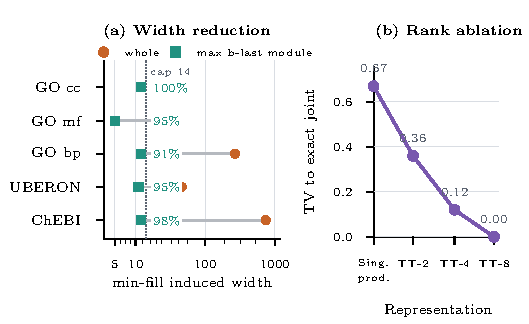
\includegraphics[width=\columnwidth]{fig_width_rank.pdf}
\caption{Structural and representation diagnostics. (a)
Unrestricted min-fill width before and after the structural pre-screen.
(b) TT-SVD representation error on one exactly enumerated 10-variable GO
cc separator.}
\label{fig:width-rank-appendix}
\end{figure}

\begin{table}[t]
\centering
\small
\setlength{\tabcolsep}{6pt}
\begin{tabular}{lrr}
\toprule
Ontology & Product TV & Product MAE \\
\midrule
GO cc  & 0.0215 & \(6.96{\times}10^{-3}\) \\
GO mf  & 0.0000 & \(3.85{\times}10^{-8}\) \\
GO bp  & 0.0003 & \(4.66{\times}10^{-5}\) \\
UBERON & 0.0000 & \(6.71{\times}10^{-7}\) \\
ChEBI  & 0.0000 & \(4.45{\times}10^{-10}\) \\
\bottomrule
\end{tabular}
\caption{Median product representation error on 15 exact-reference
instances per ontology.}
\label{tab:separator-rank}
\end{table}

\paragraph{Definition-composition diagnostic.}
The completed leak-free 16-term definition-based noisy-OR study is a
separate definition-composition diagnostic. Its all-term AUC spans
\(0.594\)--\(0.909\) across namespace--backbone settings, with
molecular-function reach identifying the operating regime of definition
composition.

\section{Application Note}
The separator-factor inference layer maps independent predictor scores
\(p_i\) to ontology-conditioned marginals \(\mu_i\) without retraining the
base predictor. A deployment specifies a compatible ontology vocabulary,
the score-calibration protocol, and the construction and TT rank used for
each approximate \(F_j\).

\section{Ontology Instantiation Details}\label{app:multi-ontology}

\paragraph{Reproducibility identifiers.}
The GO experiments use Gene Ontology release 2021-11-16. The UBERON
experiments use \texttt{uberon-basic.owl} release 2026-06-19. The ChEBI
experiments use ChEBI OBO data-version 252, dated 2026-05-01. The artifact
manifest records source paths, source URLs, and SHA256 checksums. The main
tables retain live terms and map \texttt{is-a} edges to implications
\(y_c\Rightarrow y_\pi\); the separate GO NF2 stress test adds normalized
conjunctions.

\paragraph{Structure and modular inference protocol.}
For each ontology row in the structure and operational-scale analyses, we
compute term count, edge count,
multi-parent fraction, maximum in-degree, \(\widehat w(G_T)\),
\(\widehat w(C)\), core size, number of peripheral modules,
\(\max_j\widehat w_j^\partial\), structural low-width coverage, and wall
time. The modular selector uses Algorithm~\ref{alg:core-selection}.

\paragraph{Validation protocol.}
On sampled modules small enough for enumeration, the junction-tree marginal is checked against brute force under the same local unary plug-in. On monolithic GO cc, where \(\widehat w(G_T)=12\), BP is compared directly against exact junction-tree WMC. The former check validates the local solver; agreement with global WMC is assessed by monolithic comparisons and exact dense tables for \(F_j\).

\paragraph{Baseline protocol.}
DeepProbLog-style exact compilation is evaluated on increasing GO bp
subgraphs under the common resource protocol. Scallop is evaluated with
proof-provenance semantics on 200 GO bp neighborhoods and top-\(k\) values
\(k\in\{1,2,3,5,10,20,50\}\). A-NeSI and NeSyDM are contextual
learned-inference comparisons on carry chains. The same-semantics main
tables use brute force, junction-tree inference, PySDD, mini-bucket, loopy
BP, and modular WMC with the shared Boolean theory and literal weights.

\section{Formalisation: implementation and lemma inventory}\label{app:lean}

\paragraph{A kernel-checked development with decidable rational arithmetic.}
The Lean~4 development (\texttt{Wmc.lean}, Lean 4.31) is a single Lean-core file with no
dependence on \texttt{mathlib}. It defines worlds as Boolean lists, the true-path constraint
as a conjunction of edge clauses $(\neg y_c \vee y_\pi)$, the exact weighted model count as a
ratio of summed world weights (\texttt{marginal}), and the soft-OR update (\texttt{softOR}),
and it closes every claim by \texttt{decide}, reduction in the kernel, with no
\texttt{native\_decide} escape hatch and therefore no trust placed in compiled code. To keep
rational arithmetic cheap in the kernel we use a \emph{custom rational encoding}. A rational
is a pair $Q=\mathbb{Z}\times\mathbb{Z}$ of numerator and denominator, with addition,
multiplication and complementation ($1-a$) defined directly on the pair, and equality the
\emph{cross-multiplied} test $a_1 b_2 = b_1 a_2$, decidable on integers without normalizing the
fraction. Hence world enumeration, weighting, summation, and the soft-OR/WMC comparison are all
reducible by \texttt{decide}. \texttt{\#print axioms} reports every theorem depends on
$\{\texttt{propext}\}$ alone, with no \texttt{Classical.choice}, no \texttt{Quot.sound}, no
\texttt{sorry}.

\paragraph{Parametric development and lemma inventory.}
The general Theorem~\ref{thm:star}, over all $k:\mathbb{N}$ and all real priors, is proved in a
separate \texttt{mathlib} development (\texttt{WmcStar.star\_marginal\_eq\_softOR}, Lean 4.31).
It models worlds as \texttt{Bool}\,$\times$\,(\texttt{Fin}\,$k\to$\texttt{Bool}), uses the
product-of-sums interchange \texttt{Finset.prod\_univ\_sum} to evaluate the parent-true mass to
$q_\pi$ and \texttt{Finset.sum\_eq\_single} to collapse the parent-false case to the all-false
world, giving $Z=q_\pi+(1-q_\pi)\prod_i(1-q_i)$ and the soft-OR ratio. Its axiom footprint is
$\{\texttt{propext},\texttt{Classical.choice},\texttt{Quot.sound}\}$ with no \texttt{sorry}. The
concrete Lean-core development additionally checks the instances directly. The single edge
(\texttt{single\_edge\_exact}) and the $k{=}2,3$ stars (\texttt{star2\_exact},
\texttt{star3\_exact}) reduce both sides to the same $Q$ by \texttt{decide}. The reconvergence is the diamond
($d\!\Rightarrow\!b,c$, $b,c\!\Rightarrow\!a$). \texttt{diamond\_exact\_5\_6} proves the exact
reconvergent marginal is $5/6$. \texttt{diamond\_softor\_9\_10} proves the soft-OR update (the
two paths merged independently) is $9/10$. \texttt{diamond\_softor\_ne\_exact} proves they
are unequal. These lemmas prove the star identity and the path-independent diamond failure.
The deployed synchronous damped loopy BP on cyclic graphs is evaluated
empirically in the reconvergence diagnostics and GO cc exact-reference
comparison.

\section{Extended neuro-symbolic comparison numbers}\label{app:nesy}

\paragraph{Top-$k$ provenance (Scallop).}
The four-node reconvergent derivation has two proof paths to a shared fact via the upward rule $\texttt{holds}(P)\!:\!-\,\texttt{sub}(C,P),\texttt{holds}(C)$ at edge-probability $\tfrac12$, a construction distinct from the Lean true-path diamond in the theoretical analysis (different inference semantics, so its exact value $0.9375$ does not conflict with $5/6$ on that diamond). Run in the actual Scallop system (\texttt{scallopy}, built from source, top-$k$-proofs), the exact marginal $P(\texttt{holds}(a))=0.9375$ is returned as $0.50$ at $k{=}1$ (a $47\%$ undercount), $0.875$ at $k{=}3$, and the exact $0.9375$ at $k{=}10$, identical to our exact-semantics reference. On real biological-process neighbourhoods the maximum drift versus the exact provenance reference falls from $0.34$ at $k{=}1$ (over 200 targets, $0.21$ on a $14$-term cone run in \texttt{scallopy}) to below $10^{-3}$ at $k{=}10$. The error therefore grows with proof multiplicity (reconvergence) and shrinks as $k$ admits more proofs, the same reconvergence axis along which loopy BP departs from exact $\WMC$.

\paragraph{The carry-chain: exact independence vs.\ its sampled estimate.}
We instantiate the $N$-digit carry chain as MNIST addition under distant (sum-only) supervision,
training a shared digit CNN with the independence-assumption marginal of the sum and reporting
test sum-accuracy over three seeds. With the \emph{exact} independence product (computed by
convolving the per-position digit distributions) the model degrades only gently as the carry
couples more digits: $0.970/0.942/0.926/0.905$ for $N{=}1$ to $4$, with gradual compounding
of per-digit error. Its bare \emph{Monte-Carlo} estimate, the sampling a naive
learned objective rests on, collapses over the same range, $0.129/0.010/0.001/0.000$,
as the probability that a sample satisfies the constraint vanishes and the gradient disappears.
This is the independence-assumption / reasoning-shortcut failure
\citep{vankrieken2024independence,marconato2023reasoningshortcuts} addressed by learned inference
engines. On the same benchmark, A-NeSI ($20$ epochs/seed) gives sum-accuracy
$0.973/0.922/0.875/0.748$ from $N{=}1$ to $4$. Its degradation tracks the exact product because A-NeSI learns an inference distribution; direct constraint sampling exhibits the collapse above. This shifts the cost to task-specific training: applying A-NeSI or NeSyDM
\citep{vankrieken2025nesydm} to GO would require a model trained per ontology, and A-NeSI would
also require samples from the exact $\WMC$ target.

\paragraph{TT-rank representation dial on a GO cc upper cone.}
The exact constraint-induced joint distribution over the variables in a real GO cc upper cone ($10$ terms, $53$ models, exact tensor-train rank $6$) is strongly non-product. Exhaustive enumeration followed by TT-SVD dials the tensor reconstruction residual to zero as rank increases. This experiment evaluates representation capacity alone; scalable construction of \(F_j\) and posterior recovery inside modules are evaluated separately. The rank-$1$ product approximation and the implemented loopy BP produce distinct outputs.

\begin{table}[t]\centering
\caption{TT-SVD representation error on one exactly enumerated GO cc upper cone with 10 terms. $q^\star$ is the exact constraint-induced joint distribution. ``Gap closed'' is the fraction of the rank-$1$ total variation removed.}\label{tab:rank}
\footnotesize
\setlength{\tabcolsep}{3pt}
\begin{tabular}{@{}lccc@{}}
\toprule
Boundary head & KL & TV & Gap closed\\
\midrule
rank-$1$ (indep.) & $1.95$ & $0.68$ & -- \\
rank-$2$ & $1.46$ & $0.36$ & $46\%$\\
rank-$4$ & $0.26$ & $0.12$ & $82\%$\\
rank-$6$ (full) & $0.00$ & $0.00$ & exact\\
\bottomrule
\end{tabular}
\end{table}

\paragraph{The dial is systematic across cores.}
Over 40 deterministically selected high-degree multi-parent cc upper cones of up to 13 terms, the
constraint-induced joint distribution is non-product in every case. The IA gap
$\mathrm{KL}(q^\star\Vert\text{product})$ is $1.49$ nats in the median (range $0.54$--$3.75$).
The exact rank of the joint is $5$ in the median (range $3$--$10$), always far below the $2^{w}$
dense size. The example in Table~\ref{tab:rank} is the first cone meeting the fixed size criterion;
the aggregate distribution, not this single example, is the relevant evidence.

\paragraph{The disjunctive (SROIQ) regime: a multimodal joint.}
On a controlled fragment over $w{=}6$ boundary atoms, two entities, each typed by
an exactly-one-of-three axiom (covering $+$ pairwise disjointness), coupled by cross-entity
disjointness, the exact joint is \emph{multimodal} ($6$ modes), and the IA cannot represent it.
The best product discards $2.03$ nats (total variation $0.87$, $11\%$ error on a composed query). The
rank-$r$ dial is exact only at full rank $3$ of the joint (Table~\ref{tab:disj}). This is the
regime that the disjoint-cube result of van Krieken rules out for the IA, and the one a SROIQ extension targets.

\begin{table}[t]\centering
\caption{Cost-II in the disjunctive (SROIQ) regime: covering $+$ disjointness over $w{=}6$ atoms give a $6$-mode joint distribution the IA cannot represent. A rank-$r$ representation is exact at full rank $3$. ``WMC rel.\ err.'' is the relative error on a composed query $P(a_1\vee b_2)$.}\label{tab:disj}
\footnotesize
\setlength{\tabcolsep}{3pt}
\begin{tabular}{@{}lccc@{}}
\toprule
Boundary model & KL & TV & WMC rel.\ err.\\
\midrule
IA (best product) & $2.03$ & $0.87$ & $1.1{\times}10^{-1}$\\
rank-$2$ & $0.38$ & $0.28$ & $4.1{\times}10^{-2}$\\
rank-$3$ (full) & $0.00$ & $0.00$ & $0$\\
\bottomrule
\end{tabular}
\end{table}

\fi
\end{document}
